% -*- mode : latex; coding: utf-8 -*-
\chapter{Discussion and Future Work}
\label{sec:optimization}

\section{Performance Trade-off Analysis}

MPU protection provides significant security benefits that justify the measured 990-cycle region allocation overhead (7.6× vs baseline):

\textbf{Security Benefits}:
\begin{itemize}
    \item Hardware-enforced bounds checking prevents buffer overflow attacks
    \item Stack overflow protection eliminates ECU reliability vulnerabilities
    \item Fault containment localizes failures to prevent total system corruption
    \item ISO 26262 functional safety support for ASIL C/D systems
\end{itemize}

\textbf{Cost-Benefit Analysis}: Hardware MPU (5.5 μs initialization overhead) significantly outperforms software protection (50-100 μs initialization + runtime overhead) while providing stronger isolation guarantees.

\section{Optimization Strategies}

Several techniques can further reduce MPU overhead:

\begin{table}[h]
\centering
\caption{MPU Optimization Potential}
\begin{tabular}{@{}lcc@{}}
\toprule
Strategy & Cycles Saved & Final Overhead \\
\midrule
Baseline (measured) & - & 990 cycles \\
Lazy Reconfiguration & 50-100 & ~900 cycles \\
Region Caching & 100-200 & ~800 cycles \\
Batch Operations & 30-80 & ~920 cycles \\
\textbf{Combined Optimizations} & \textbf{150-300} & \textbf{690-840 cycles} \\
\bottomrule
\end{tabular}
\end{table}

\begin{figure}[h]
\centering
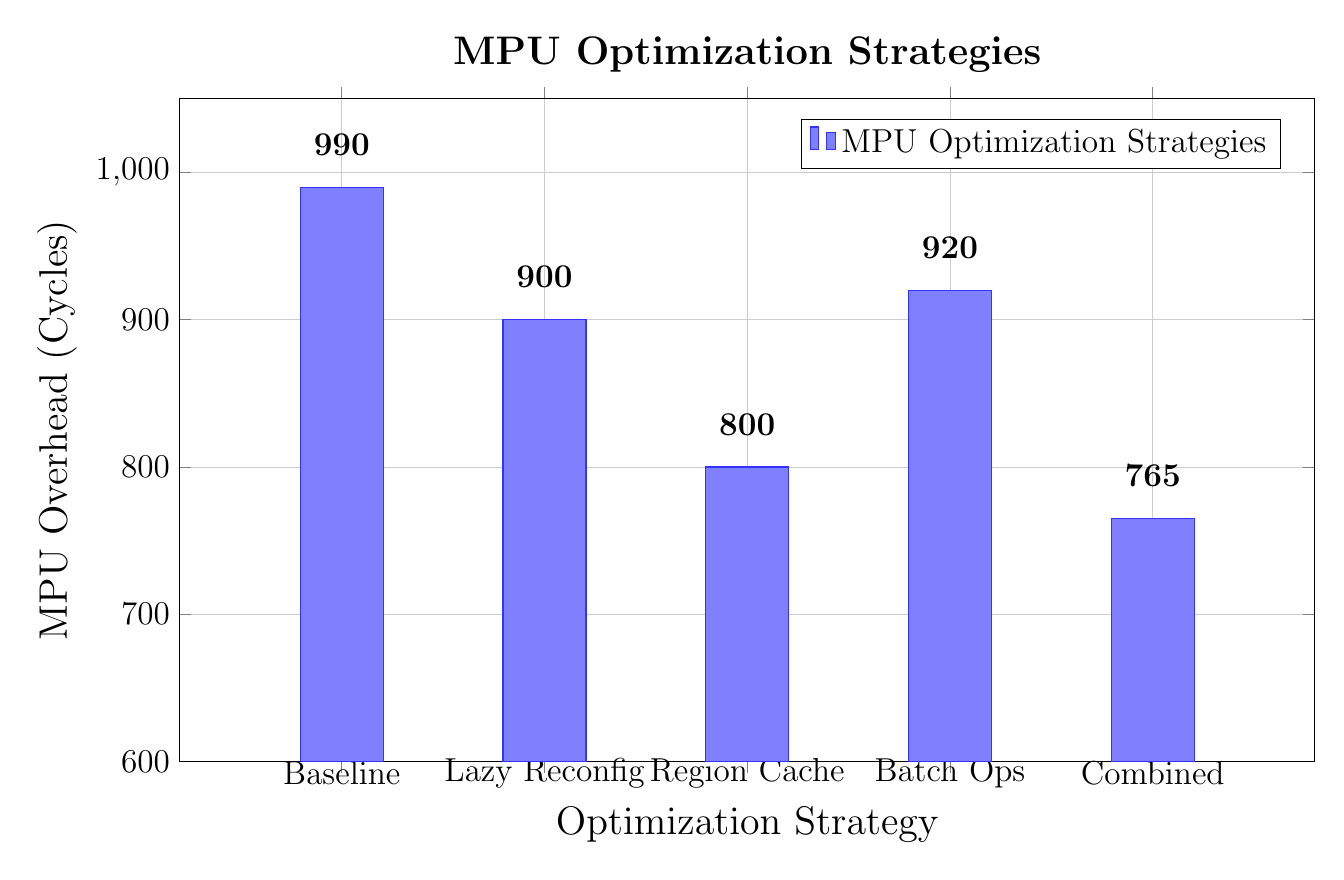
\begin{tikzpicture}
\begin{axis}[
    ybar,
    bar width=30pt,
    width=16cm,
    height=10cm,
    xlabel={\Large Optimization Strategy},
    ylabel={\Large MPU Overhead (Cycles)},
    ymin=600, ymax=1050,
    symbolic x coords={Baseline,Lazy Reconfig,Region Cache,Batch Ops,Combined},
    xtick=data,
    x tick label style={rotate=0, anchor=center, font=\large},
    tick label style={font=\large},
    label style={font=\Large},
    grid=major,
    grid style={line width=0.3pt, draw=gray!40},
    legend pos=north east,
    legend style={font=\large},
    enlarge x limits=0.2,
    title={\Large\textbf{MPU Optimization Strategies}}
]

% Simplified bar chart with consistent colors
\addplot[ybar, fill=blue!50, draw=blue!80, bar width=30pt]
coordinates {(Baseline,990) (Lazy Reconfig,900) (Region Cache,800) (Batch Ops,920) (Combined,765)};

% Add clean value labels
\node at (axis cs:Baseline,1005) [above] {\large\textbf{990}};
\node at (axis cs:Lazy Reconfig,915) [above] {\large\textbf{900}};
\node at (axis cs:Region Cache,815) [above] {\large\textbf{800}};
\node at (axis cs:Batch Ops,935) [above] {\large\textbf{920}};
\node at (axis cs:Combined,780) [above] {\large\textbf{765}};

\legend{\large MPU Optimization Strategies}
\end{axis}
\end{tikzpicture}
\caption{MPU Optimization Strategy Performance Impact}
\label{fig:optimization_potential}
\end{figure}

\vspace{1cm}

\section{Automotive Implementation Recommendations}

\begin{table}[h]
\centering
\caption{Automotive MPU Implementation Guidelines}
\begin{tabular}{@{}lccc@{}}
\toprule
ECU Category & ASIL Level & Recommended Protection & Performance Impact \\
\midrule
Engine Control & B/C & 2 MPU tasks & 0.61\% (11.0 μs) \\
Chassis Control & C/D & 2 MPU tasks & 0.12\% (11.0 μs) \\
Body Electronics & A/B & 2 MPU tasks & 0.01\% (11.0 μs) \\
Gateway/Firewall & All & Enhanced MPU + optimization & < 0.1\% \\
\bottomrule
\end{tabular}
\end{table}

\section{Limitations and Future Work}

\textbf{Current Limitations}:
\begin{itemize}
    \item Single platform focus (STM32F446RE-specific results)
    \item Synthetic workloads may not capture all automotive complexity
    \item Static analysis approach requires dynamic optimization investigation
\end{itemize}

\textbf{Future Directions}:
\begin{enumerate}
    \item Multi-platform validation across automotive microcontroller families
    \item Production application analysis with OEM collaboration
    \item Security effectiveness study through penetration testing
    \item AI-driven optimization for adaptive MPU configuration
\end{enumerate}